\chapter{Project Analysis} 

\section{Problem definition}

\paragraph{}
Today, the health data that we can access through the internet is quite large. However, due to the data pollution in this area, people may think that they are	caught	in	a	deadly	illness when	they	search	for	a	complaint	they	are	experiencing	on	the	internet.	Even	diseases	that require	long-term	examination	and	detailed	analysis	to	be	diagnosed	can	easily	be	presented to	people.	What's	more,	there	are	many	forums	that	bring	doctors	and	people	together	on	the	internet,	as	well	as	sites	that	function	as	an	individual	dialogue.	On	these	pages,	people	can	ask	irrelevant	or	absurd	questions	to	doctors	because	of	wrong	information	or	ignorance. 

\section{Decision Support System}

\paragraph{}
As our decision making is based on the database, so the facts we possess we can say that our Decision Support System is knowledge-driven. Thanks to out Telegram Bot use, our application is interactive and easy to use.

\paragraph{Decision Support System definition}:\\
$Input: symptoms + personal\ data$\\
$Output: 3\ most\ probable\ diseases\ along\ with\ advices$\\
$Boundary: Limited\ by\ the\ database$\\
$Processes: Compute\ score\ on\ diseases\ depending\ input\ data$\\
$Decision\ makers: Maximum\ score\ reached\ OR\ Maximum\ number\ of\ questions\ reached\ OR\ Set\ of\ chosen\ diseases\ small\ enough$\\


\section{SWOT Analysis}

\begin{figure}[H]
	\centering
	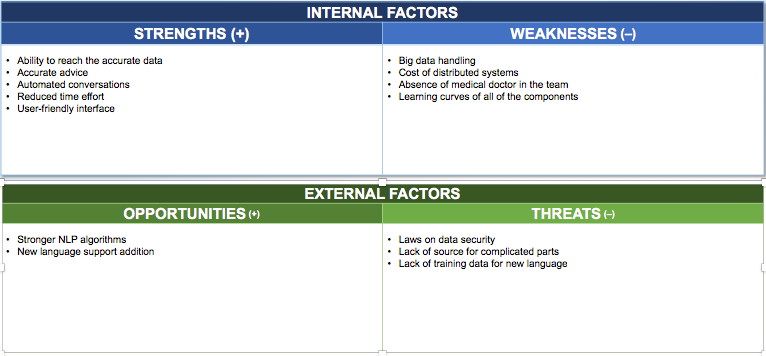
\includegraphics[width=\textwidth]{swot}
	\caption{SWOT Analysis}
	\label{swot}
\end{figure}

\section{Division of labor}

We did not have an experience in the chatbot field, and because of our lack of experience in python	tools, we did the work part in accordance with the principle of volunteering. In this context we divided the different tasks as showed on table \ref{labor}.
\begin{table}[H]
	\centering
	\begin{tabular}{|c|p{10cm}|}
		\hline
		\textbf{Group member} & \textbf{Labor} \\
		\hline
		Emirhan	Kutlu & Django back-end, ChatterBot usage and integration, Telegram chat bot programming and competitive and SWOT Analysis \\
		\hline
		Lucie Labadie & Django back-end, Multi-classifier with SciKit-learn and documentation, supervision report \\
		\hline
		Rosen Sasov & Public database search, Database architectural design and front-end \\
		\hline
	\end{tabular}
	\caption{Division of labor}
	\label{labor}
\end{table}	

Apart from these, collaborated studies and meetings	were held to decide on the method needed for diagnosis.